%\setcounter{chapter}{13} % "N" (14th letter, but latex first increments -> 14-1=13)
\chapter{Synchronization Method} \label{ch:sync}


Reliable OFDM communication relies heavily on maintaining orthogonality between subcarriers.
In a real acoustic environment, hardware imperfections and channel propagation introduce time delays and frequency offsets that destroy this orthogonality.
Consequently, before any demodulation or channel estimation can occur, the receiver must perform a rigorous synchronization process.
This chapter details the implemented techniques for packet detection, frequency correction, and phase tracking \autocite{Schmidl1997}.

\section{Time Synchronization (Packet Detection)} \label{sec:TimeSync}

The first stage of the receiver pipeline is to identify the precise start of the data packet within the incoming stream of samples.
This is achieved using a known \textbf{Preamble} sequence prepended to the frame.
The function \texttt{estimateTauAndCFO} implements a normalized cross-correlation algorithm to locate this sequence.

Mathematically, the timing metric $M(d)$ at delay $d$ is computed as:
\begin{equation}
    M(d) = \frac{|\sum_{n=0}^{L-1} r^*[d+n] p[n]|^2}{\sum_{n=0}^{L-1} |r[d+n]|^2},
\end{equation}
where $r[n]$ is the received signal, $p[n]$ is the known preamble, and $L$ is the preamble length.
Normalization by the received energy (the denominator) is crucial to ensure the thresholding mechanism remains robust against varying volume levels in the acoustic channel.

As shown in \Cref{fig:correlation_metric}, the algorithm searches for a peak in $M(d)$ that exceeds a predefined threshold (\texttt{conf.preamble.thr}).
Once the peak is detected, the index is refined to pinpoint the exact sample marking the end of the preamble and the beginning of the payload.

\begin{figure}[!ht]
    \fcapside[\FBwidth]{%
        \captionsetup{parskip = .5\baselineskip plus 1pt}%
        \caption[Frame Detection Metric]{%
            Signal magnitude (top) and normalized correlation metric (bottom) used for frame detection.
            The distinct peak in the correlation metric $M(d)$ identifies the precise synchronization point $\tau$ despite the noisy received amplitude.
        }%
        \label{fig:correlation_metric}%
    }{%
        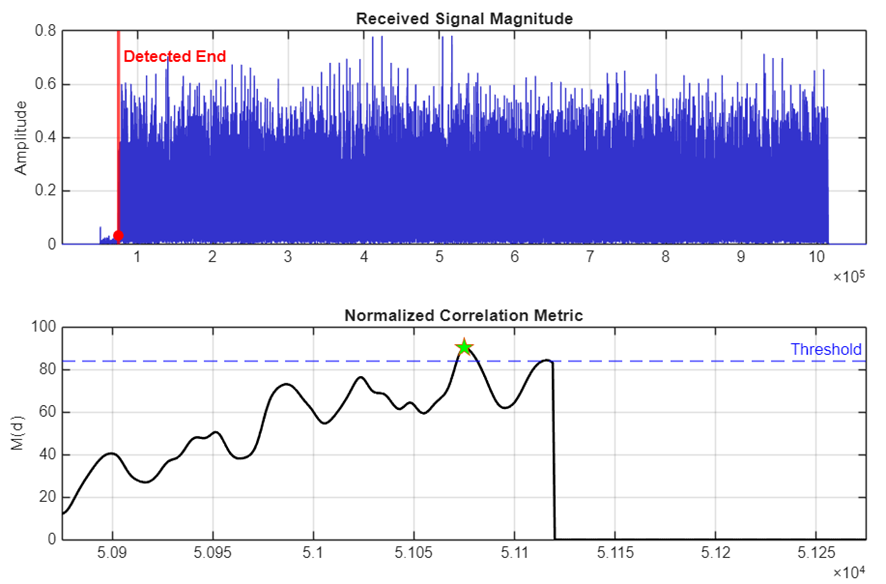
\includegraphics[width=0.60\textwidth]{figures/chap3_channel/c4_5.png}
    }
\end{figure}

\section{Frequency Synchronization (CFO Estimation)} \label{sec:FreqSync}

Oscillator mismatches between the transmitter (laptop) and receiver (microphone) introduce a Carrier Frequency Offset (CFO).
Left uncorrected, CFO causes a progressive phase rotation of the constellation symbols, leading to Inter-Carrier Interference (ICI).
The system mitigates this via a two-stage estimation process embedded in \texttt{estimateTauAndCFO}:

\begin{enumerate}
    \item \textbf{Coarse Estimation:} A grid search is performed over a range of potential frequency offsets (defined in \texttt{ofdmc.rangeCFO}). The system de-rotates the received preamble by each candidate frequency and computes the correlation. The frequency yielding the maximum response is selected as the coarse estimate.
    \item \textbf{Fine Estimation:} To achieve sub-grid precision, the system applies quadratic interpolation (parabolic fitting) around the coarse peak. This estimates the true maximum of the correlation function, providing a highly accurate CFO value.
\end{enumerate}

The entire received signal is then multiplied by $e^{-j2\pi \Delta f t}$ to compensate for the estimated offset $\Delta f$.

\section{Channel Estimation and Pilots} \label{sec:PilotsTraining}

Once synchronized, the receiver must compensate for the channel's spectral distortion.
The frame structure includes a dedicated \textbf{Training Symbol} located immediately after the preamble.
This symbol contains known values on all active subcarriers.
By comparing the received training symbol to the transmitted reference, the Least Squares (LS) estimator computes the initial Channel Frequency Response (CFR), as detailed in \Cref{ch:channel}.

\subsection{Phase Tracking with Pilots}
While the Training Symbol provides a snapshot of the channel at the beginning of the frame, residual CFO or slow channel variations can cause the phase to drift over the duration of the packet.
To counter this, \textbf{Pilot Symbols} are inserted into specific subcarriers (e.g., indices defined in \texttt{ofdmc.pilotIndices}) of every OFDM data symbol.

The function \texttt{correctOFDMSymbolRotation} extracts these pilots after equalization.
It computes the residual phase rotation $\theta_m$ for the $m$-th OFDM symbol by averaging the phase difference between the received pilots and the known transmitted pilots.
This per-symbol correction ensures the constellation remains stable throughout the transmission, preventing the "spinning" effect common in uncorrected OFDM systems.

\section{Cyclic Prefix (CP)} \label{sec:CP}

To combat multipath propagation—clearly visible in the taps of \Cref{fig:trans_cir_pdp} (Appendix)—a \textbf{Cyclic Prefix} is prepended to every OFDM symbol.
The CP acts as a guard interval, absorbing the Inter-Symbol Interference (ISI) caused by delayed echoes.
Crucially, it converts the linear convolution of the channel into a circular convolution, which is the mathematical prerequisite (\autocite{NeePrasad2000}) for simple single-tap equalization in the frequency domain.

As discussed in \Cref{ch:channel}, the length of the CP determines the maximum delay spread the system can tolerate.
While a conservative length (e.g., 256 samples) ensures robustness in reverberant rooms (Channel 5), it reduces spectral efficiency.
Adaptive CP scaling remains a viable optimization for benign channels (Channels 1 and 2). This will also be analyzed in detail in \Cref{ch:transmission} for each channel.